\chapter{Normalisasi Teks dengan Jarak Perubahan}

\section{Alur Pengerjaan Tugas Akhir}

Alur pengerjaan Tugas Akhir ini dapat dilihat pada Gambar \ref{fig:alur_pengerjaan}. Pengerjaan Tugas Akhir melibatkan empat tahap, yaitu identifikasi masalah, tinjau pustaka, perancangan, dan pengujian. Tahap-tahap dalam pengerjaan Tugas Akhir dijelaskan sebagai berikut:
\begin{enumerate}
	\item identifikasi masalah, yaitu melakukan sebuah identifikasi untuk menentukan permasalahan yang akan diselesaikan dalam pengerjaan Tugas Akhir, yang mana permasalahan tersebut adalah normalisasi terhadap kata tidak baku yang tidak disingkat;
	\item tinjau pustaka, yaitu melakukan peninjauan referensi yang terkait dengan pengerjaan Tugas Akhir serta menjadikan referensi tersebut sebagai acuan perbandingan, yaitu referensi \parencite{saragih2017normalisasi}. Selain itu, dilakukan peninjauan algoritme yang akan dipilih sebagai usulan, yaitu algoritme jarak Levenshtein dan jarak Jaro-Winkler;
	\item perancangan, yaitu melakukan rancangan masukan, proses, dan keluaran yang diharapkan sebagai usulan untuk metode normalisasi dalam pengerjaan Tugas AKhir;
	\item pembangunan, yaitu melakukan pembangunan terhadap metode normalisasi usulan dalam pengerjaan Tugas Akhir; dan
	\item pengujian, yaitu melakukan perbandingan antara metode normalisasi yang berasal dari referensi \parencite{saragih2017normalisasi} dengan metode normalisasi usulan.
\end{enumerate}
\begin{figure}[ht]
	\centering
	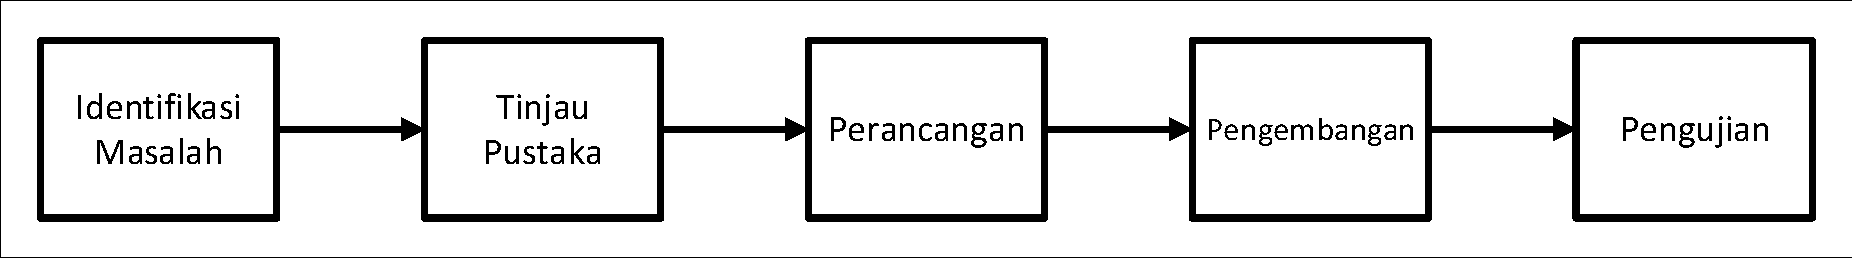
\includegraphics[width=\textwidth, trim=2 2 2 2, clip]{resources/3/alur_pengerjaan.pdf}
	\caption{Alur pengerjaan Tugas Akhir}
	\label{fig:alur_pengerjaan}
\end{figure}

\section{Alur Proses Normalisasi Teks dengan Jarak Perubahan}

Rancangan untuk keseluruhan metode normalisasi teks usulan terdapat dalam Gambar \ref{fig:ta_sistem}. Metode normalisasi teks usulan memiliki tiga bagian utama, yaitu bagian masukan, proses, dan keluaran.
\begin{figure}[ht]
	\centering
	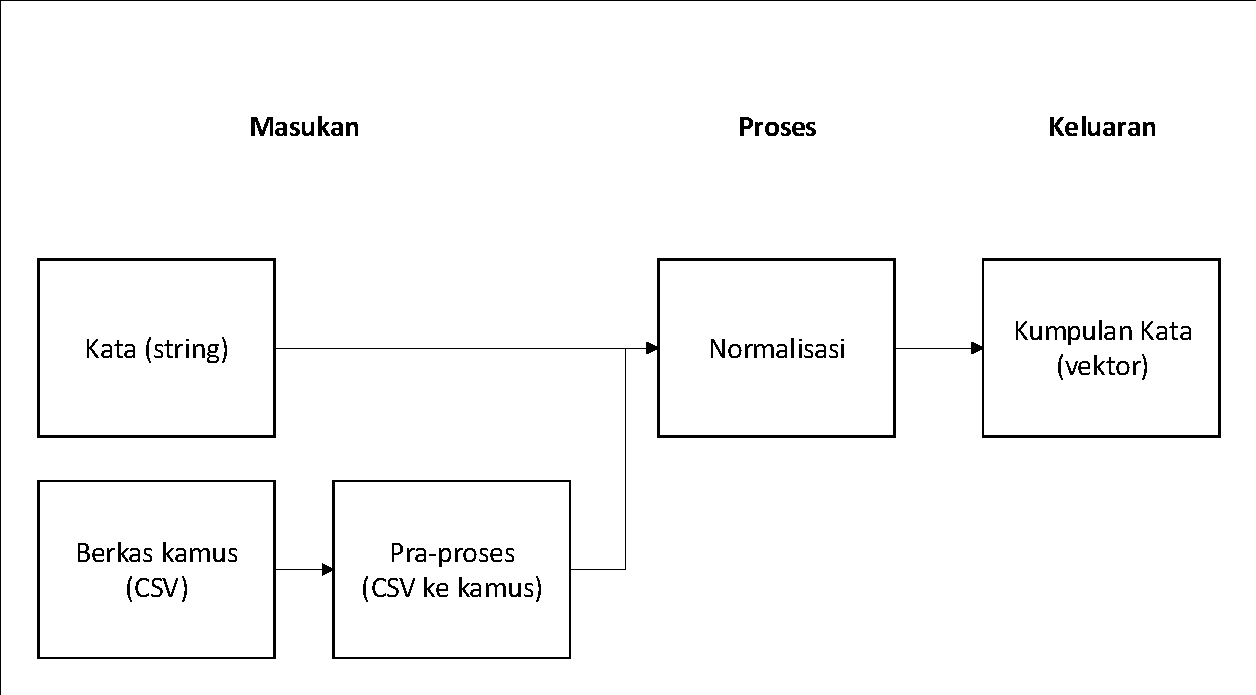
\includegraphics[width=\textwidth, trim=2 2 2 2, clip]{resources/3/ta_sistem.pdf}
	\caption{Alur metode normalisasi teks}
	\label{fig:ta_sistem}
\end{figure}

\subsection{Bagian Masukan Normalisasi Teks}

Metode normalisasi usulan memiliki dua jenis masukan, yaitu kata dan kamus kata baku. Kedua masukan diperlukan sehingga metode normalisasi dapat mencari kemiripan antara kata masukan dengan kamus kata baku. Kedua masukan metode dijelaskan sebagai berikut:
\begin{enumerate}
	\item masukan kata, yaitu sebuah \textit{string} mengandung kata tidak baku yang berasal dari masukan pengguna. Contoh dari masukan kata seperti "\textit{asem}", "\textit{puter}", dan lain-lain; dan
	\item masukan berkas kamus, yaitu kumpulan kata-kata yang berasal dari kamus kata baku dalam bentuk berkas CSV. Sebelum dapat digunakan, berkas CSV harus melalui pra-proses berupa konversi berkas CSV menjadi kamus yang dapat digunakan oleh metode normalisasi.
\end{enumerate}

\subsection{Bagian Proses Normalisasi Teks}

Gambar \ref{fig:side_to_side} bagian (a) menunjukkan alur proses untuk rancangan metode normalisasi yang diusulkan. Metode normalisasi usulan menggunakan jarak Levenshtein sebagai penghitungan jarak antara kedua teks. Deskripsi alur proses yang dijalankan dapat dijelaskan sebagai berikut:
\begin{enumerate}
	\item diberikan kata masukan dan kamus kata baku,
	\item melakukan pencarian kata-kata dalam kamus kata baku yang memiliki kemiripan yang tinggi dengan kata masukan, menghasilkan kumpulan kata, dan,
	\item melakukan seleksi kata yang menjadi kata keluaran. Jika terdapat lebih dari satu kata, maka kata yang dipilih adalah kata yang pertama kali ditemukan.
\end{enumerate}
\begin{figure}[ht]
	\centering
	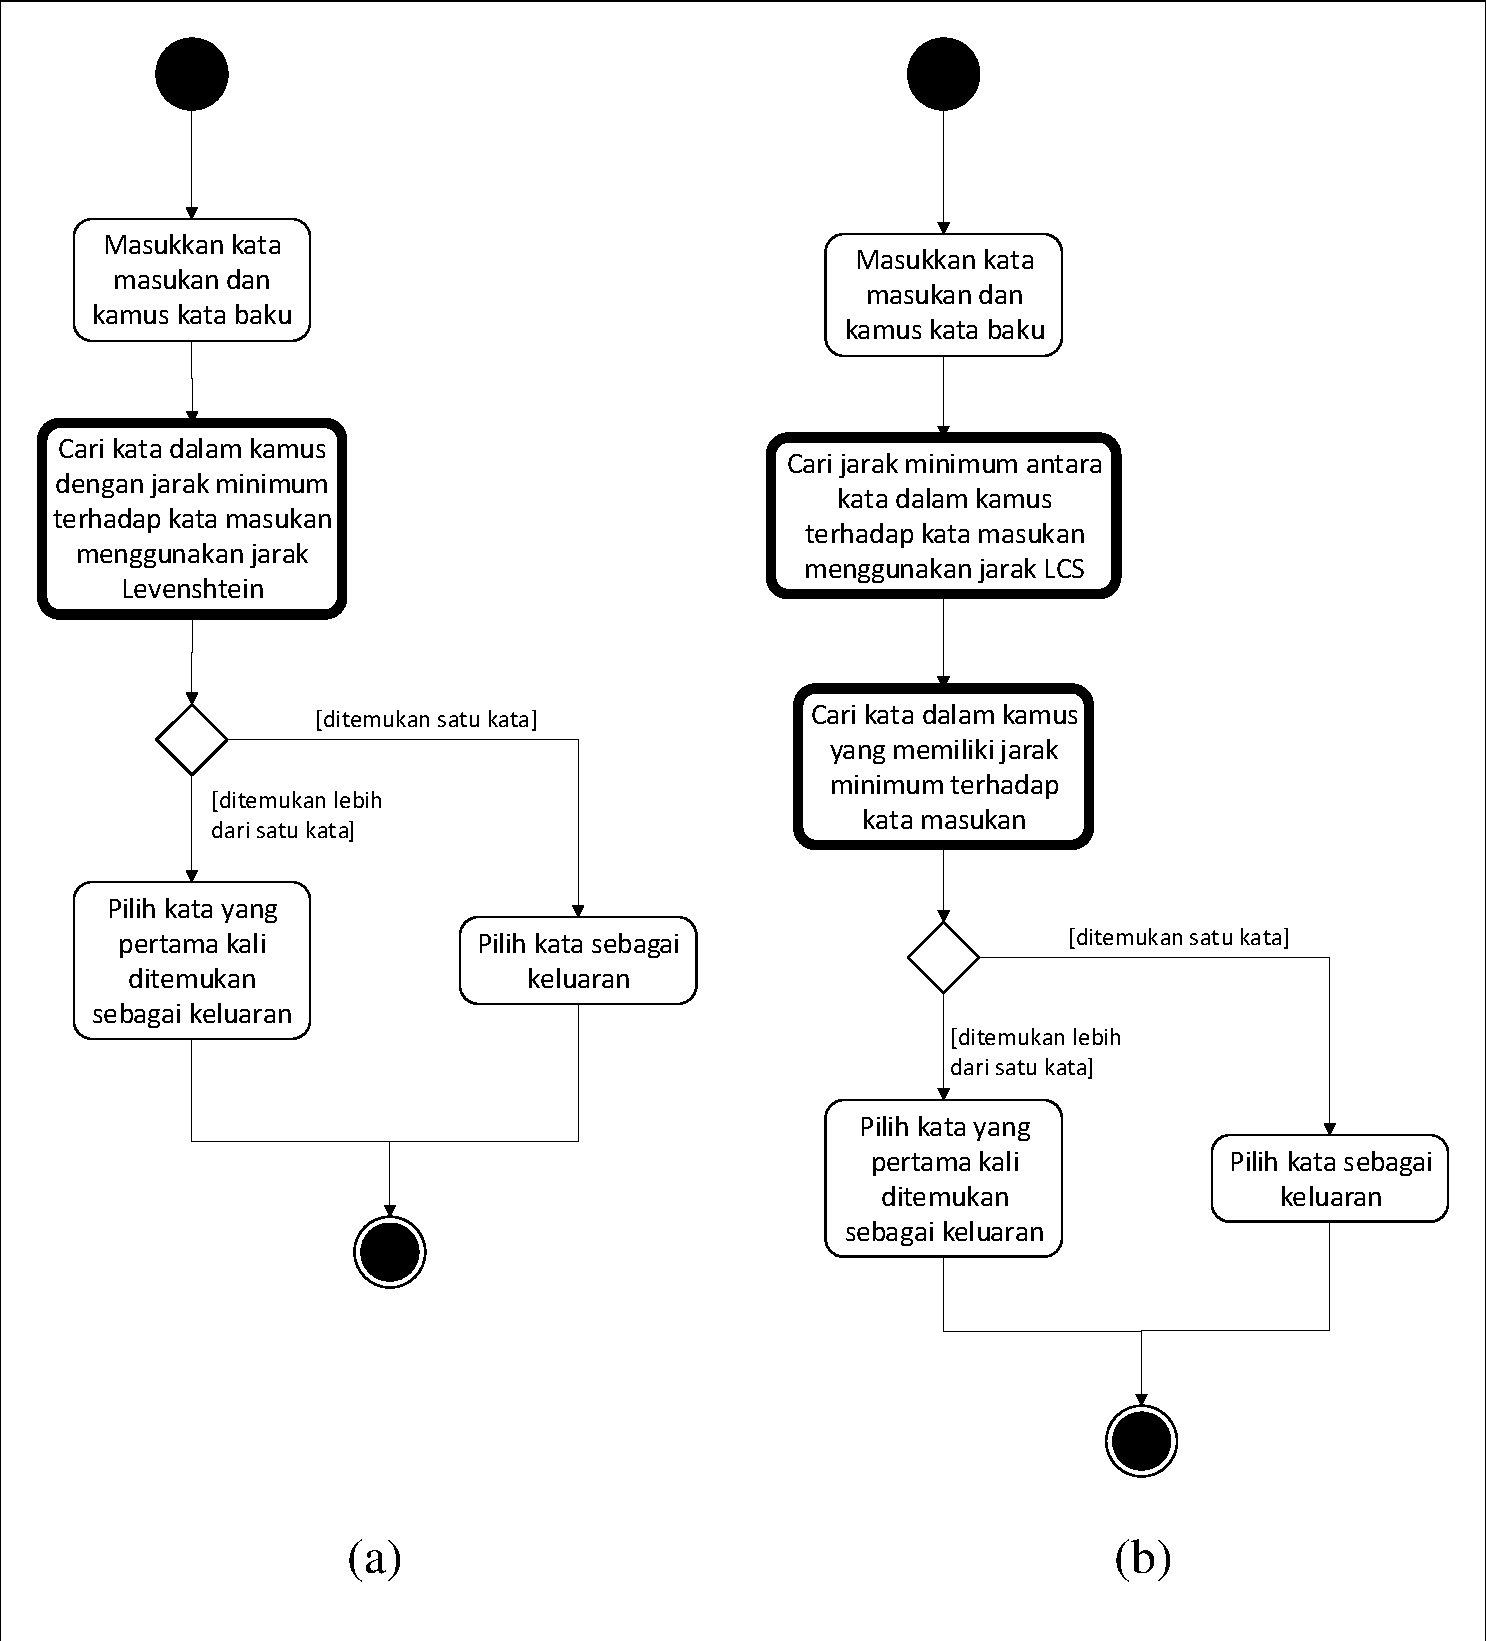
\includegraphics[width=0.8\textwidth, trim=2 2 2 2, clip]{resources/3/side_to_side.pdf}
	\caption{Alur proses normalisasi teks dengan (a) metode usulan, dan (b) metode \parencite{saragih2017normalisasi}}
	\label{fig:side_to_side}
\end{figure}

Terdapat perbedaan alur proses antara metode normalisasi \parencite{saragih2017normalisasi} dengan metode normalisasi usulan. Perbedaan tersebut dapat dilihat pada blok proses dengan garis tepi tebal pada Gambar \ref{fig:side_to_side}. Perbedaan pertama terletak pada penggantian algoritme jarak LCS dengan algoritme usulan, yaitu jarak Levenshtein dan jarak Jaro-Winkler. Kedua, metode normalisasi usulan mempersingkat proses normalisasi dengan menemukan kumpulan kata prediksi dengan jarak minimum secara langsung dibandingkan metode normalisasi \parencite{saragih2017normalisasi} yang harus mencari jarak minimum terlebih dahulu kemudian menemukan kumpulan kata prediksi dengan jarak tersebut.

\subsubsection{Algoritme Jarak Levenshtein}

Algoritme \ref{lst:lv} merupakan algoritme persamaan jarak Levenshtein yang dapat dilihat pada Rumus \ref{eq:lv} \parencite{levenshtein1966binary}. Algoritme menerima masukan berupa dua kata dan mengeluarkan nilai jarak perubahan berupa bilangan bulat. Penghitungan jarak perubahan kedua kata masukan dilakukan dengan menggunakan matriks dua dimensi dengan ukuran matriks disesuaikan dengan kedua masukan kata tersebut.
\begin{lstlisting}[caption={Algoritme Fungsi Jarak Levenshtein},label={lst:lv},float,floatplacement=H]
Masukan: str1, str2		: string
Keluaran: integer

Deklarasi:
str1, str2 				: string
len1, len2, i, j, actv 	: integer
matrix					: array[][] integer

Deskripsi:
Mulai
1. Menambah str1 dan str2 dengan spasi di depan;
2. masukkan secara berurutan nilai panjang str1 dan str2 ke dalam variabel len1 dan len2;
3. membuat matrix dengan ukuran len1 x len2 lalu isi semua sel dengan nilai 0;
4. selama i diantara 1 dan len1 - 1, isi sel matrix[i][0] dengan nilai i;
5. selama j diantara 1 dan len2 - 1, isi sel matrix[0][j] dengan nilai j;
6. selama i diantara 1 dan len1 - 1 dan j diantara 1 dan len2 - 1:
	a) masukkan variabel actv dengan nilai 1;
	b) jika str1[i] sama dengan str2[j], ubah nilai actv dengan nilai 0;
	c) masukkan variabel matrix[i][j] dengan nilai terkecil antara matrix[i-1][j] + 1, matrix[i][j-1] + 1, atau matrix[i-1][j-1] + actv.
7. keluarkan nilai dalam variabel matrix[len1-1][len2-1].
Selesai
\end{lstlisting}

\subsubsection{Algoritme Jarak Jaro-Winkler}

Algoritme \ref{lst:jw} \parencite{orsiniumtext} merupakan algoritme persamaan jarak Jaro-Winkler yang dapat dilihat pada Rumus \ref{eq:jaro} dan Rumus \ref{eq:jw}. Algoritme menerima masukan berupa dua kata dan mengeluarkan nilai jarak perubahan berupa bilangan bulat. Penghitungan kemiripan kedua kata masukan dilakukan dengan menghitung rata-rata dari ketiga pembagian yang ada di dalam algoritme, lalu melakukan perkalian dengan faktor skala dan panjang \textit{common string} yang digunakan.
\begin{lstlisting}[caption={Algoritme Fungsi Jarak Jaro-Winkler \parencite{orsiniumtext}},label={lst:jw},float,floatplacement=H]
	Masukan: s1, s2	: string, prefix_weight = 0.1 : float
	Keluaran: float
	
	Deklarasi:
	s1, s2 							: string
	s1_len, s2_len, common_chars, i	: integer
	weight, prefix_weight			: float
	
	Deskripsi:
	Mulai
	1. Masukkan secara berurutan nilai panjang s1 dan s2 ke dalam s1_len dan s2_len;
	2. hitung jumlah karakter yang sesuai, lalu masukkan nilainya ke common_chars;
	3. hitung jumlah transposisi yang terjadi, bagi dengan dua, lalu masukkan nilainya ke trans_count;
	4. hitung rata-rata dari common_chars/s1_len, common_chars/s2_len, dan (common_chars-trans_count)/common_chars, lalu masukkan nilainya ke weight;
	5. masukkan nilai j dengan nilai terkecil antara min_len dan empat (4);
	6. hitung nilai i dengan jumlah karakter awal yang sesuai, maksimal bernilai empat;
	7. kalikan i, prefix_weight, dan 1-weight, jumlahkan dengan nilai weight, lalu masukkan nilainya ke weight;
	8. keluarkan nilai weight.
	Selesai
\end{lstlisting}

\subsubsection{Algoritme Normalisasi Teks Usulan}

Fungsi dalam Algoritme \ref{lst:lv} dan Algoritme \ref{lst:jw} digunakan untuk metode normalisasi kata pada Algoritme Normalisasi Teks Usulan dengan tujuan untuk mencari kumpulan kata baku yang memiliki kemiripan dengan kata masukan. Algoritme tersebut dibedakan satu sama lain dikarenakan perbedaan keluaran antara Levenshtein dan Jaro-Winkler, yang mana Levenshtein mengeluarkan jarak perubahan berbentuk bilangan bulat dan Jaro-Winkler mengeluarkan tingkat kemiripan berbentuk bilangan desimal.

\begin{enumerate}[label=\textit{\Alph*)}, itemindent=*, series=process_list]
	\item Algoritme Normalisasi Kata dengan Jarak Levenshtein
\end{enumerate}

Algoritme normalisasi kata dengan jarak Levenshtein, ditunjukkan oleh Algoritme \ref{lst:lev_find}, bertujuan untuk mencari kumpulan kata yang memiliki jarak perubahan paling kecil dengan menggunakan jarak Levenshtein. Terdapat dua masukan metode yaitu sebuah kata dan sebuah kamus dalam bentuk vektor. Metode menghasilkan dua keluaran, yaitu nilai jarak terkecil antara kata masukan dengan seluruh kata dalam kamus dan vektor berisi kumpulan kata dengan jarak terkecil dengan kata masukan.
\begin{lstlisting}[caption={Algoritme Fungsi Normalisasi Kata dengan Jarak Levenshtein},label={lst:lev_find},float=ht]
Masukan: txt : string, kam : dictionary
Keluaran: array, integer

Deklarasi:
txt, word		: string
val, minVal 	: integer
kam				: dictionary
similarWords	: array[] string

Deskripsi:
Mulai
1. Masukkan nilai 30 ke dalam variabel minVal;
2. masukkan nilai txt ke dalam vektor similarWords;
3. untuk seluruh kata dalam kam:
	a) Masukkan nilai kata ke dalam variabel word;
	b) hitung jarak Levenshtein antara txt dengan word, simpan hasil ke dalam variabel val;
	c) jika val lebih kecil dari minVal:
		i) jika val sama dengan nol (0), jadikan word sebagai vektor lalu keluarkan vektor bersama dengan nilai 0;
		ii) jika val tidak sama dengan nol, ganti similarWords dengan vektor berisi word lalu ganti minVal dengan val.
	d) jika val sama dengan minVal, tambah nilai ke dalam array similarWords.
4. keluarkan array similarWords dan nilai dalam variabel minVal.
Selesai
\end{lstlisting}

Berbagai kondisional yang tercantum dalam Algoritme \ref{lst:lev_find} dijelaskan sebagai berikut:
\begin{enumerate}
	\item "jika \textit{val} sama dengan nol (0)" yaitu kata masukan (\textit{txt}) dan kata dalam kamus (\textit{word}) adalah kata yang sama persis, ditunjukkan dengan jarak perubahan (\textit{val}) bernilai nol. Oleh karena itu, \textit{word} langsung diubah menjadi vektor lalu dijadikan sebagai keluaran fungsi beserta nilai jaraknya yaitu nol;
	\item "jika \textit{val} tidak sama dengan nol" yaitu ditemukan \textit{word} dengan jarak yang lebih kecil dibandingkan jarak terkecil (\textit{minVal}) sebelumnya sehingga seluruh isi vektor kumpulan kata (\textit{similarWords}) terdahulu harus dibuang lalu digantikan dengan \textit{word}; dan
	\item "jika \textit{val} sama dengan \textit{minVal}" yaitu ditemukan \textit{word} yang memiliki jarak yang sama dengan seluruh kata dalam \textit{similarWords} sehingga \textit{word} harus dimasukkan ke dalam \textit{similarWords}.
\end{enumerate}

\begin{enumerate}[resume*=process_list]
	\item Algoritme Normalisasi Kata dengan Jarak Jaro-Winkler
\end{enumerate}

Algoritme normalisasi kata dengan jarak Jaro-Winkler, ditunjukkan oleh Algoritme \ref{lst:jw_find}, bertujuan untuk mencari kumpulan kata yang memiliki kemiripan paling tinggi dengan menggunakan jarak Jaro-Winkler. Terdapat dua masukan metode yaitu sebuah kata dan sebuah kamus dalam bentuk vektor. Metode menghasilkan dua keluaran, yaitu nilai kemiripan antara kata masukan dengan seluruh kata dalam kamus dan vektor berisi kumpulan kata dengan nilai kemiripan dengan kata masukan.
\begin{lstlisting}[caption={Algoritme Fungsi Normalisasi Kata dengan Jarak Jaro-Winkler},label={lst:jw_find},float=ht]
	Masukan: txt : string, kam : dictionary
	Keluaran: array, float
	
	Deklarasi:
	txt, word		: string
	val, maxVal 	: float
	kam				: dictionary
	similarWords	: array[] string
	
	Deskripsi:
	Mulai
	1. Masukkan nilai 0 ke dalam variabel maxVal;
	2. masukkan nilai txt ke dalam vektor similarWords;
	3. untuk seluruh kata dalam kam:
		a) Masukkan nilai kata ke dalam variabel word;
		b) hitung jarak Jaro-Winkler antara txt dengan word, simpan hasil ke dalam variabel val;
		c) jika val lebih besar dari maxVal:
			i) jika val sama dengan satu (1), jadikan word sebagai vektor lalu keluarkan vektor bersama dengan nilai 1;
			ii) jika val tidak sama dengan satu, ganti similarWords dengan vektor berisi word lalu ganti maxVal dengan val.
		d) jika val sama dengan maxVal, tambah nilai ke dalam array similarWords.
	4. keluarkan array similarWords dan nilai dalam variabel maxVal.
	Selesai
\end{lstlisting}

Berbagai kondisional yang tercantum dalam Algoritme \ref{lst:jw_find} dijelaskan sebagai berikut:
\begin{enumerate}
	\item "jika \textit{val} sama dengan satu (1)" yaitu kata masukan (\textit{txt}) dan kata dalam kamus (\textit{word}) adalah kata yang sama persis, ditunjukkan dengan nilai kemiripan (\textit{val}) bernilai 1. Oleh karena itu, \textit{word} langsung diubah menjadi vektor lalu dijadikan sebagai keluaran fungsi beserta nilai kemiripannya yaitu satu;
	\item "jika \textit{val} tidak sama dengan satu" yaitu ditemukan \textit{word} dengan nilai kemiripan yang lebih besar dibandingkan nilai kemiripan terbesar (\textit{maxVal}) sebelumnya sehingga seluruh isi vektor kumpulan kata (\textit{similarWords}) terdahulu harus dibuang lalu digantikan dengan \textit{word}; dan
	\item "jika \textit{val} sama dengan \textit{maxVal}" yaitu ditemukan \textit{word} yang memiliki nilai kemiripan yang sama dengan seluruh kata dalam \textit{similarWords} sehingga \textit{word} harus dimasukkan ke dalam \textit{similarWords}.
\end{enumerate}

\subsection{Bagian Keluaran Normalisasi Teks}

Contoh keluaran metode normalisasi teks usulan tertera pada Tabel \ref{tbl:eg_output}. Salah satu contoh yang digunakan adalah kata "\textit{mikir}". Kata "\textit{mikir}", berdasarkan jarak Levenshtein, memiliki keluaran kumpulan kata-kata baku, yaitu "pikir", "bikir", "kikir", "likir", "milir", dan "zikir". Semua kata baku tersebut memiliki jarak perubahan yang sama dengan kata "\textit{mikir}" yaitu 1. Jarak tersebut juga merupakan jarak terkecil yang dapat dicapai antara kata masukan dengan seluruh kata yang ada di dalam kamus.
\begin{table}[ht]
    \captionsetup{justification=justified,singlelinecheck=false}
    \caption{Contoh keluaran Normalisasi Teks dengan Jarak Levenshtein}
    \label{tbl:eg_output}
    \centering
    \begin{tabularx}{\textwidth}{|c|X|Y|}
		\hline
		\textbf{Contoh kata} & \multicolumn{1}{Y|}{\textbf{Contoh keluaran}} & \textbf{Contoh keluaran} \\
        \textbf{masukan} & \multicolumn{1}{Y|}{\textbf{kumpulan kata}} & \textbf{jarak terkecil} \\ \hline
        \textit{mikir} & {[}'pikir', 'bikir', 'kikir', 'likir', 'milir', 'zikir'] & 1 \\ \hline
        \textit{maen} & {[}'main', 'man', 'men'] & 1 \\ \hline
        \textit{begimana} & {[}'bagaimana', 'begana']& 2 \\ \hline
    \end{tabularx}
\end{table}